\documentclass[thesis.tex]{subfiles}

\begin{document}
Neural networks have become an increasingly relevant part to data analysis, and this is also true for the XENON1T experiment \cite{Bart}.
A neural network is one section of machine learning that is heavily based off the structure of animal brains \cite{deep-learning}.
Where an animal brain is able to learn by activating specific neurons for thoughts and actions, the neurons in a machine learn in a similar vein by adjusting weights according to how wrong the machine has so far been performing \cite{deep-learning}.
The exact manner for a neural network to change these weights is done through backpropagation \cite{deep-learning}.
Backpropagation is influenced by the structure of the neural network, such as the number of neurons, how they are connected between layers, and the activation functions that are used \cite{deep-learning}.
For this reason, it is relevant for us to try alternative neural networks that have not yet been applied.

\par For our problem, the input layer will be the signal seen by the PMTs in the top array of the detector, and the output layer will be the $(x,y)$ position of the interaction.
We are mainly concerned with graph convolutional neural networks (GCNNs) which are a result of the success with convolutional neural networks (CNNs) \cite{GCNN_Kipf}.
\begin{figure}[t]
	\centering
	\begin{subfigure}{0.32\textwidth}
		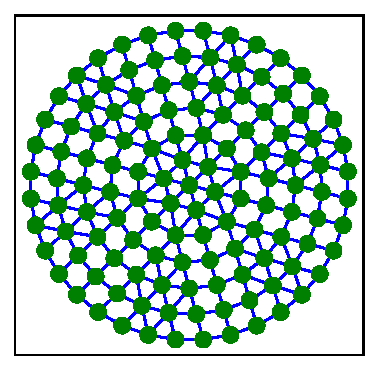
\includegraphics[width=\textwidth]{figures/1T_radius-graph_R10.pdf}
		\caption{}
	\end{subfigure}
	\begin{subfigure}{0.32\textwidth}
		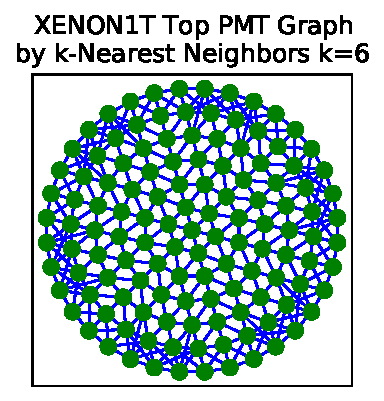
\includegraphics[width=\textwidth]{figures/1T_kNN-graph_k6.pdf}
		\caption{}
	\end{subfigure}
	\begin{subfigure}{0.32\textwidth}
		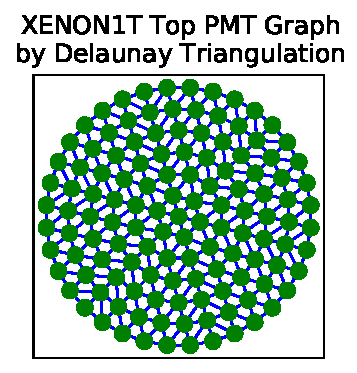
\includegraphics[width=\textwidth]{figures/1T_delaunay-graph.pdf}
		\caption{}
	\end{subfigure}
	\caption{
	Three of the considered graph structures: Radius $R=10$ cm neighbors (a), $k$-nearest-neighbors $k=6$ (b), Delaunay triangulation neighbors (c).
	Each node here is a photomultiplier tube in the top array of the XENON1T detector.
	The positions of each tube in the detector was used for each of the explored graph structure approaches.
	}
	\label{fig:graph_structs}
\end{figure}
\subsection{Convolutional Neural Networks}\label{subsec:CNN}
A convolutional neural network is a specific kind of neural network that features a convolution layer and a pooling layer \cite{deep-learning}.
The input to a CNN frequently comes in the form of a matrix where there is a locality between the elements in the matrix \cite{deep-learning}.
Many CNNs are applied to images, where pixels are the elements of the matrix.
The convolution layer makes use of a kernel that does element multiplication of weights to a submatrix of the input \cite{deep-learning}.
This is repeated as a scan over the entire matrix.
In the case of an image, smaller sections of the image pass through this kernel until all of the image is scanned.
This results in the network learning the important features of the matrix, or image.

\par However, the structure of our dataset does not have a form that can be easily made into a matrix.
The top array of PMTs has a radial formation and symmetry.
A transformation into a rectangular matrix would not preserve the locality between nearby PMTs.
Therefore, we would need an algorithm that is capable of making use of datasets with any possible structure.
\begin{figure}[t]
	\centering
	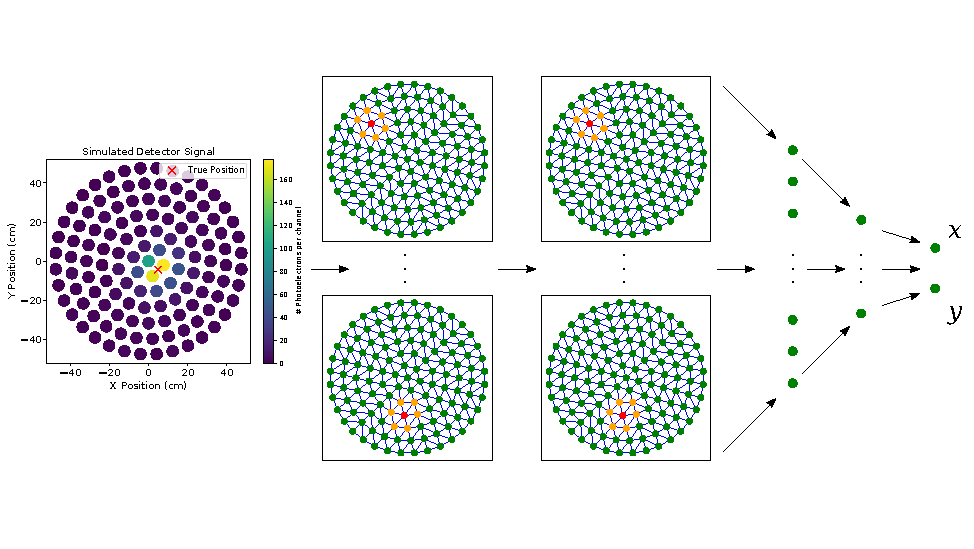
\includegraphics[width=\linewidth]{figures/gcnn_architecture.pdf}
	\caption{
	The graph convolutional neural network structure that the results of this paper are based on.
	The final structure features the signal input layer, two propagation (graph convolution) layers, two fully connected layers, and a final output layer for the $(x,y)$ position of the interaction.
	Between each layer is a ReLU activation function.
	There are a total of 57,486 trainable parameters.
	}
	\label{fig:figures/GCNN_Structure}
\end{figure}
\subsection{Graph Convolutional Neural Networks}\label{subsec:GCNN}
The design of the graph convolutional neural network (GCNN) came by considering how a convolution could be applied to a graph structured dataset \cite{GCNN_Kipf}.
The graph convolution layer that we use and that was proposed by Kipf and Welling propagates the values of nodes according to the edges \cite{GCNN_Kipf}.
The value of connected nodes will increase according to the values of the connected nodes while nodes that are disconnected will see no change.
This is explained in further detail in Appendix \ref{app:GCNN-Prop}.
\begin{figure}[t]
	\centering
	\begin{subfigure}{0.45\textwidth}
		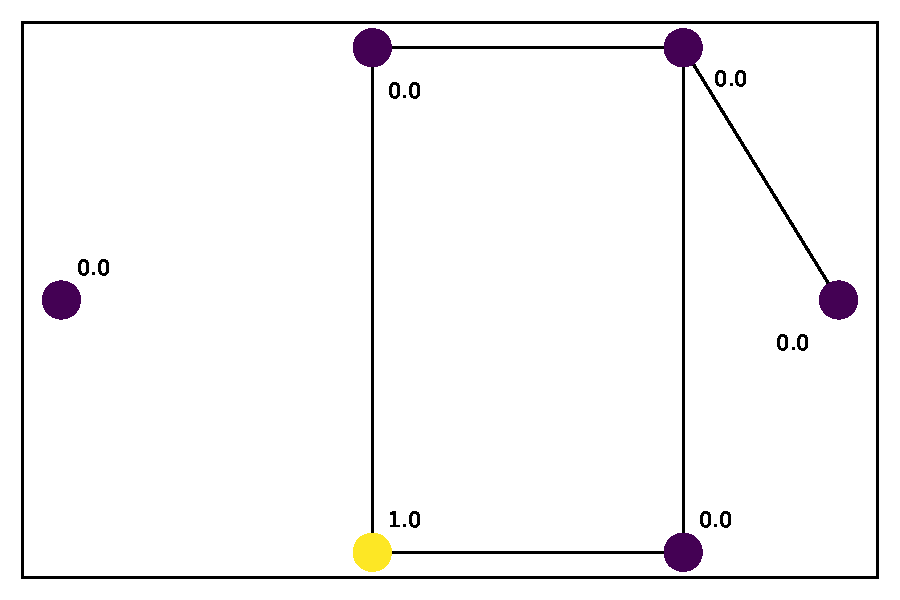
\includegraphics[width=\textwidth]{figures/graph_signal-00.pdf}
		\caption{}
		\label{fig:prop-ex-0}
	\end{subfigure}
	\begin{subfigure}{0.45\textwidth}
		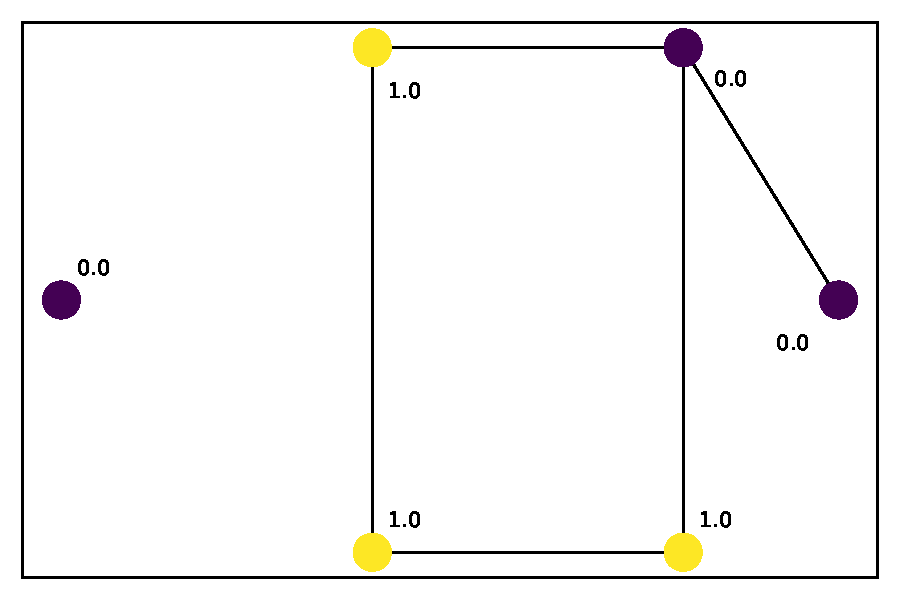
\includegraphics[width=\textwidth]{figures/graph_signal-01.pdf}
		\caption{}
		\label{fig:prop-ex-1}
	\end{subfigure}
	\begin{subfigure}{0.45\textwidth}
		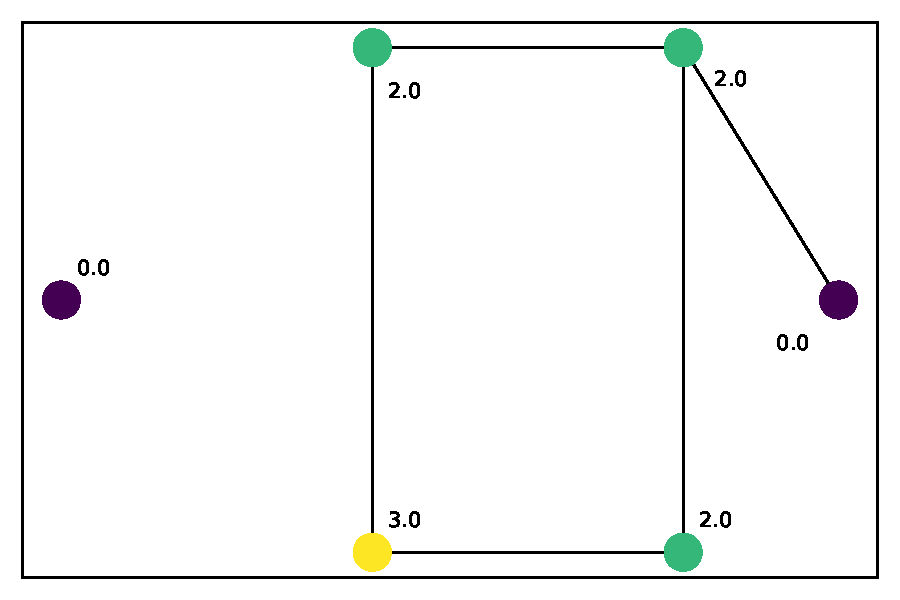
\includegraphics[width=\textwidth]{figures/graph_signal-02.pdf}
		\caption{}
		\label{fig:prop-ex-2}
	\end{subfigure}
	\begin{subfigure}{0.45\textwidth}
		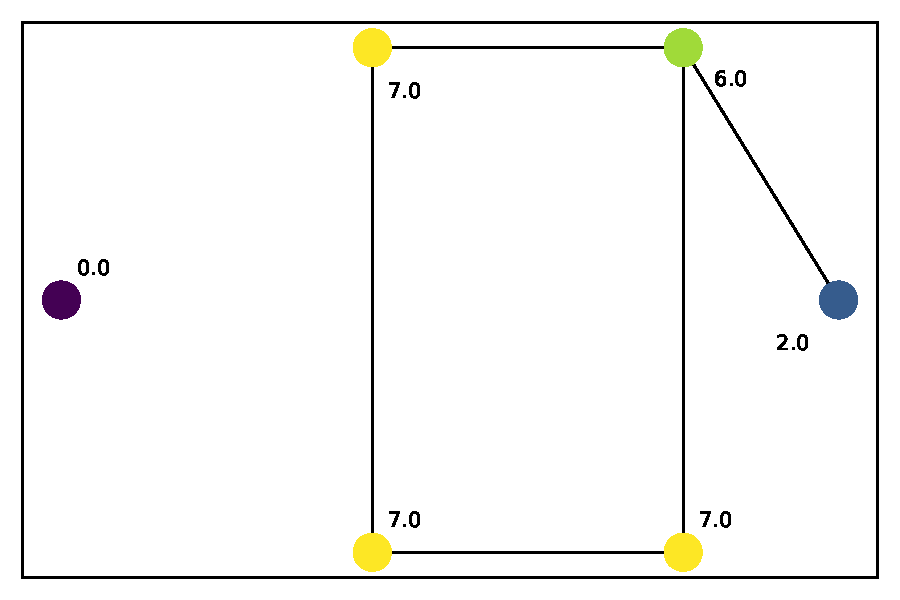
\includegraphics[width=\textwidth]{figures/graph_signal-03.pdf}
		\caption{}
		\label{fig:prop-ex-3}
	\end{subfigure}
	\caption{
	Example propagation from graph convolutions.
	The value immediately next to each node is an attribute of that node and will be passed during propagation.
	These are passed according to edges that connect each of the nodes.
	The initial signal is shown in (a), the result after the first propagation in (b), after the second propagation in (c), and after the third propagation in (d).
	}
	\label{fig:prop-ex}
\end{figure}

\par Figure \ref{fig:prop-ex} is a toy example of how a graph convolution layer propagates values.
The initial value for every node is given in Figure \ref{fig:prop-ex-0}.
The node will propagate the value of 1 to its neighbors and back to the node itself.
Since all other nodes have values of 0, there is no change otherwise.
We would expect to see three nodes with values of 1, as is shown in Figure \ref{fig:prop-ex-1}.
Continuing the propagation, results in graph in Figure \ref{fig:prop-ex-2} and one step further results in \ref{fig:prop-ex-3}.
The nodes nearest the initially high value node will also become high in value, while nodes that are further away will have a lesser value.
Nodes that are completely disconnected will see no changes.

\par We considered the PMTs of the XENON1T detector as our nodes and their quantity of light collected as their primary value.
We also included the $(x,y)$ position of the PMT at the top of the detector as addition values.
These positions are intended to provide additional weighting when learning, but the quantity of light collected will be the main factor in reconstructing the positions of events.
We chose to use rectified linear units (ReLU) as our activation function for all layers.
This function is defined as:
\begin{equation}
	\text{ReLU}\left( x \right) \equiv \text{max}\left(0,\,x\right) .
\end{equation}
This choice was to create a strict cut off for the wall of the detector.
The use of exponential linear units would not provide this strict cut off.

\par With regard to the network structure, we were influenced by the success of image classifiers, such as AlexNet \cite{AlexNet}.
However, convolutional neural networks of this structure and graph convolutional neural networks in general are more often used for classification, while we have a regression problem.
Our reasoning to use a GCNN for reconstructing the position of interactions came from being able to encode the local structure of the XENON1T detector into the dataset.
By treating the nodes of our graph as the PMTs at the top of the detector, we understood that the connections or edges that we put in place would maintain the local structure if done carefully.
We considered several graph structures shown in Figure \ref{fig:graph_structs}.
We ultimately chose the Delaunay Triangulated graph for it's consistent connection density throughout the graph: only PMTs that are immediately near each other are connected and resulted in most nodes having 6 edges.
Only nodes that represent PMTs near the wall of the detector had degrees less than 6.
There is potential for finding the graph structure that describes the detector's data best, but for this we chose to go with a heuristic approach.
\end{document}
